\chapter{Phase 3: Fein-Design und Installation/Konfiguration}
Text Phase 3 kommt hier...

\section{Package Diagram}
Das Smartwatch besitzt einige interessante Funktionen: einen präzisen Touchscreen, Apps und Widgets, etwa zum Lesen von Mails, SMS, Twitter und Facebook sowie Infos vom gekoppelten Smartphone, etwa über verpasste Anrufe und den Akkustatus.
Standard Anwendungen die mit dem Smartwatch geliefert werden, sind Uhrzeitangaben, Erinnerungsfunktionen, Kalender-Funktionalität, oder die Aktivitätserkennung. 
Klassische Anwendungen sind auch die Fitnessfunktionalitäten.
Mit der mitegelieferten API \textit{AppKit} lassen sich Apps für die SmartWatch programmieren, die eng mit dem Smartpohone zusammenarbeiten.
Die softwaretechnische Paketstruktur ist im Package \textit{Software} abgebildet.

\begin{figure}[H]
\centering\
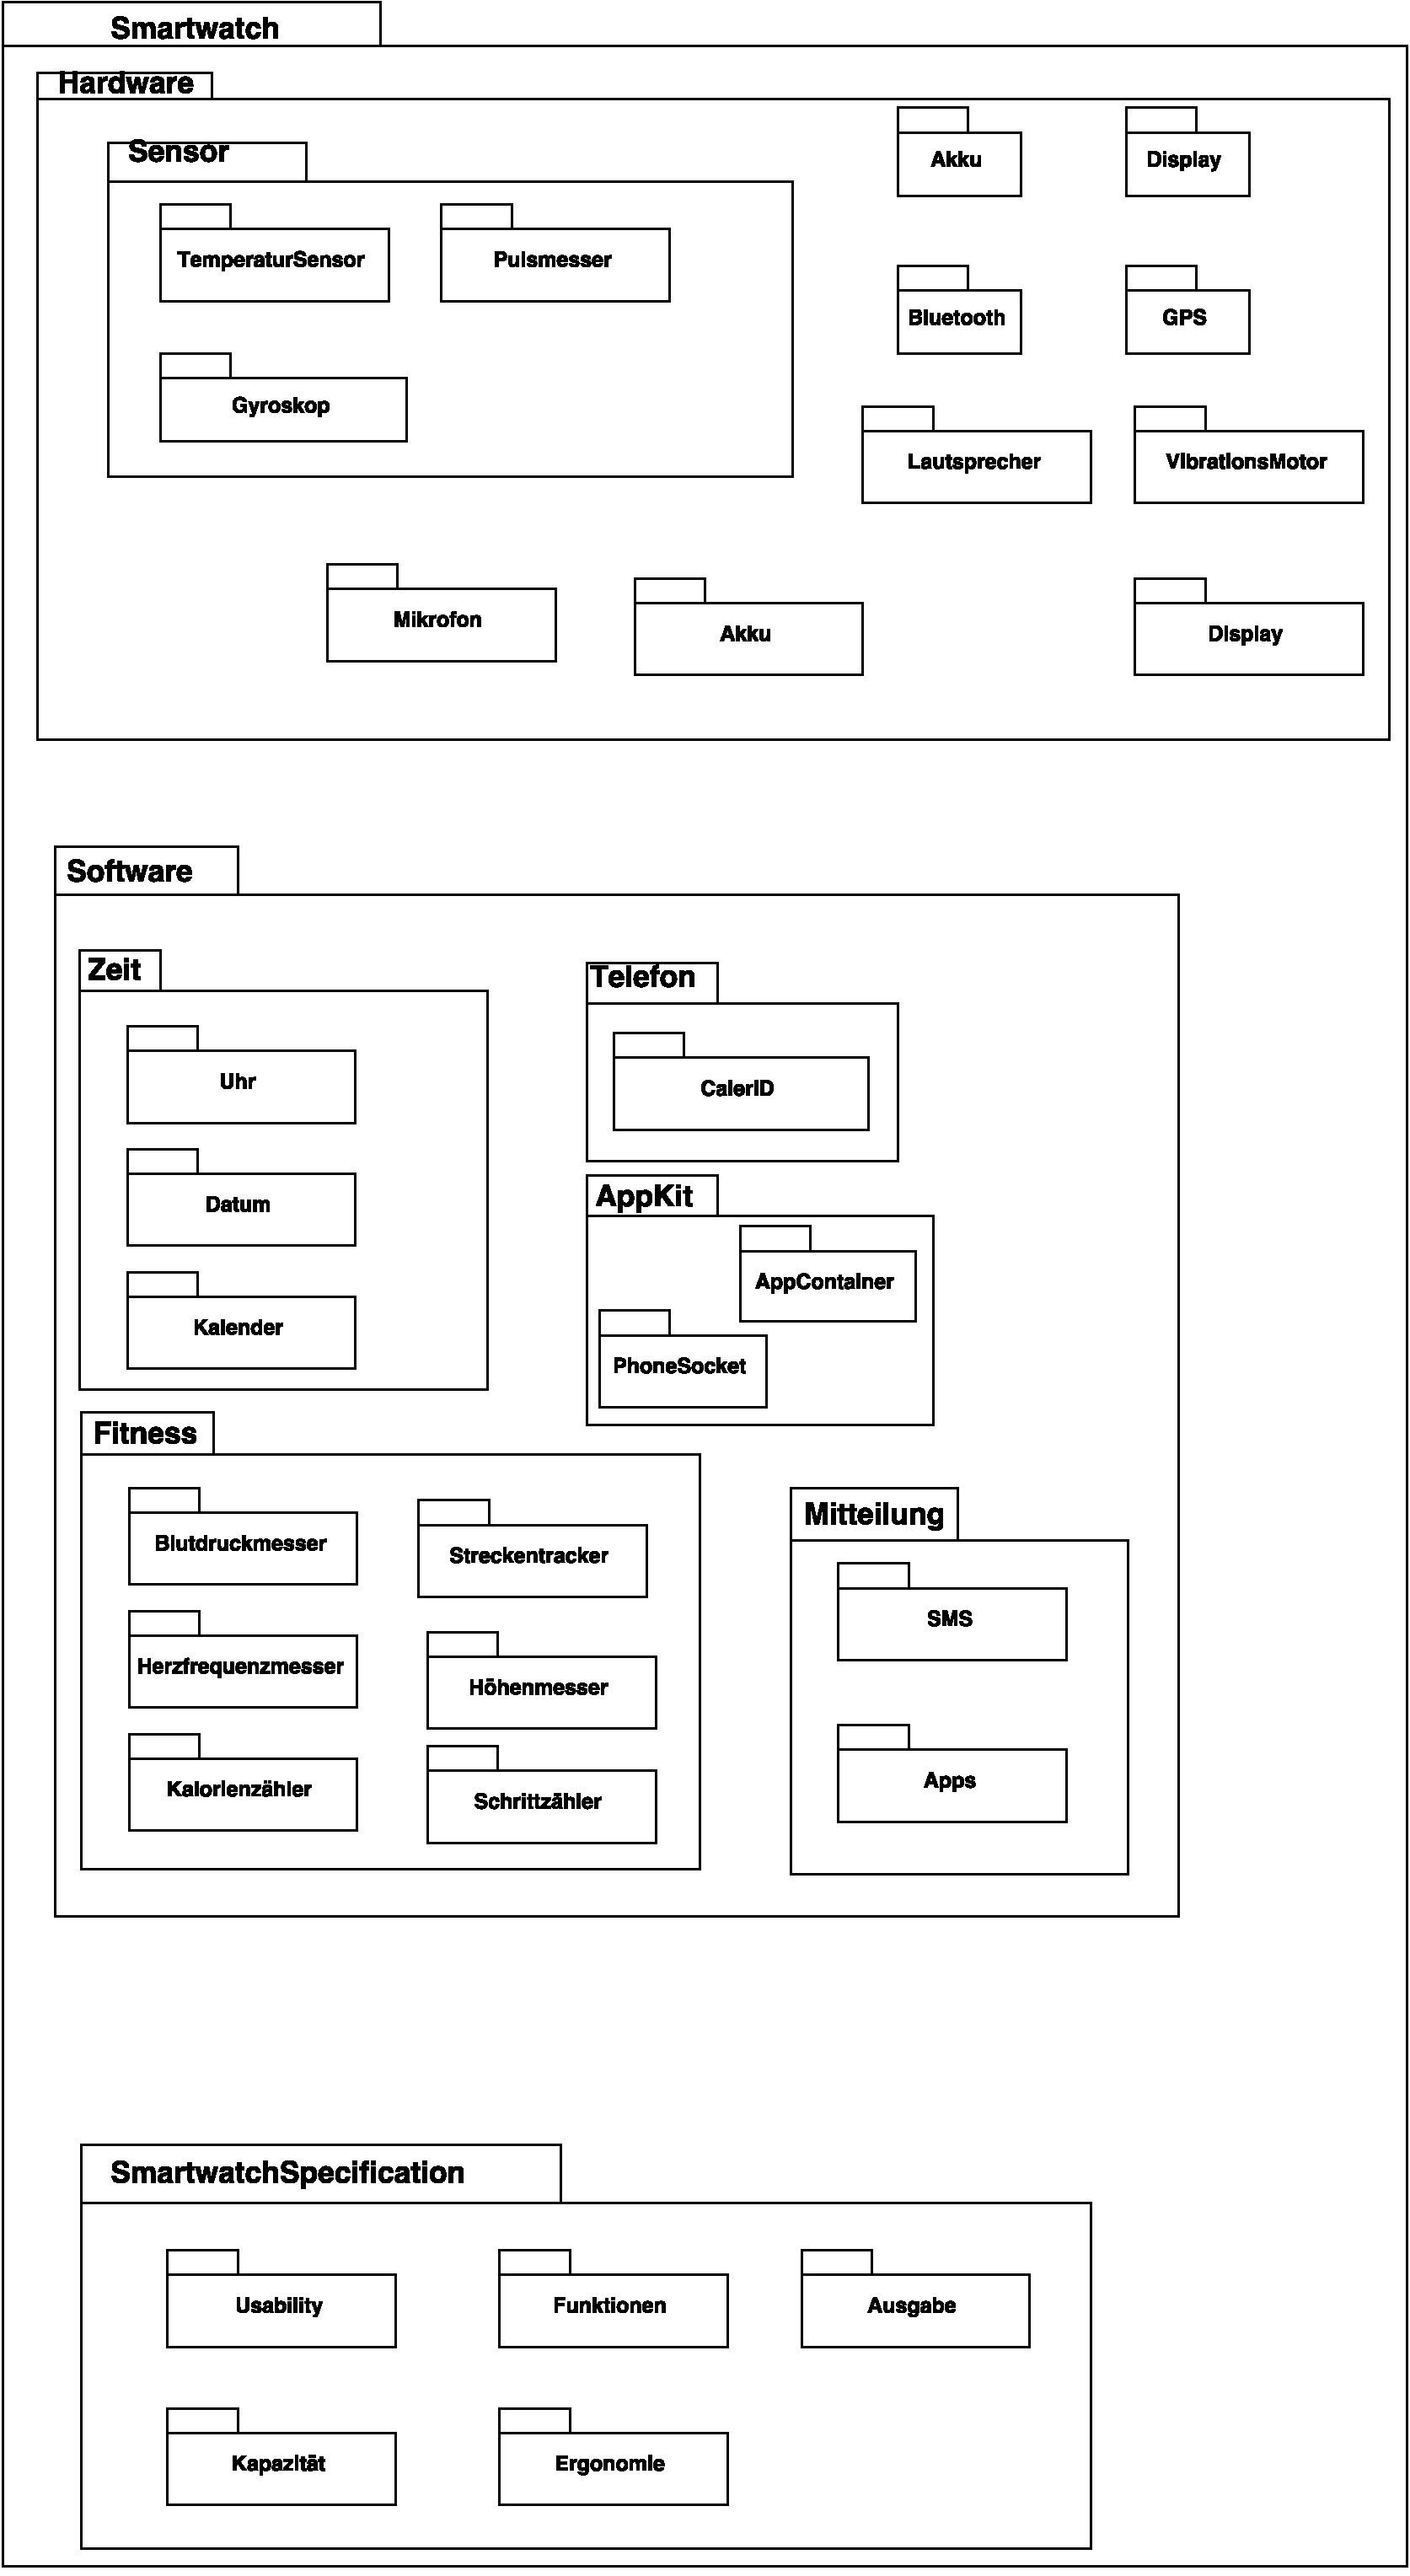
\includegraphics[width=8cm]{img/PackagePhase2}
\caption{Packetdiagramm}\label{fig:package}
\end{figure}

\section{Block Definition Diagram}

\section{Parametric Diagram}

\section{Activity Diagram}

\section{Sequence Diagram}

\section{State Diagram}
